\documentclass[11pt]{article}

\usepackage[margin=1in]{geometry}
\usepackage{setspace}
\usepackage{graphicx}
\usepackage{hyperref}
\usepackage{tikz}
\usetikzlibrary{arrows.meta, positioning}

\title{A Constitutional Framework for Non-Optimising AI Alignment}
\author{Jelbert Holtrop}
\date{10 March 2026}

\begin{document}

\maketitle

\begin{abstract}

Contemporary AI alignment approaches largely rely on optimisation. Core objectives such as safety, helpfulness, autonomy, and truthfulness are typically represented as variables within a balancing framework. While effective in many domains, such architectures share a structural vulnerability: when foundational principles become optimisable, they are susceptible to gradual reinterpretation and drift under pressure.

The constitutional model explored in this work originates from a broader philosophical framework concerned with ethical alignment grounded in principles such as unity, freedom, and compassion. The contribution of this paper, however, is not the philosophical doctrine itself.

Instead, the paper focuses on the architectural implications of embedding such principles as non-weighable constraints within an AI system. Rather than balancing foundational values against one another, the proposed framework treats them as structural boundaries that cannot be traded off or numerically optimised.

Interpretation remains necessary, but it is explicitly separated from doctrine. Drift is not assumed to be eliminated; instead, it is made detectable and classifiable through structural mechanisms such as jurisprudence and alignment auditing.

In practice, jurisprudence takes the form of documented cases that record alignment failures and establish interpretive precedents.

The central claim is architectural rather than philosophical. The paper does not argue for ethical finality. It argues that a non-optimising constitutional structure may provide greater resistance to alignment drift than optimisation-based rule aggregation.

\end{abstract}

\doublespacing

\section{The Structural Instability of Value Optimisation}

\subsection{Optimisation as the Default Paradigm}

Modern alignment systems frequently operate through balancing mechanisms. Competing objectives are weighed, implicitly or explicitly, against one another. Even when framed as constraints, these objectives often function as adjustable variables within a decision space, typically optimised through learning signals derived from human feedback \cite{christiano2017preferences}.

Balancing introduces comparison.  
Comparison introduces ranking.  
Ranking introduces optimisation.

This progression is not inherently problematic. However, it creates a structural dynamic in which foundational principles become adjustable under pressure.

\subsection{Drift as a Structural Phenomenon}

When principles are treated as comparable variables, predictable dynamics arise:

\begin{itemize}
\item Frequently reinforced behaviours dominate rare but critical cases.
\item Thresholds shift gradually.
\item Interpretations narrow for efficiency.
\item Edge cases reshape policy definitions.
\end{itemize}

Such drift does not require malicious intent. It emerges from optimisation pressure itself. Systems adapt to statistical reinforcement signals, and over time, operational meaning shifts subtly.

The core issue is not error but adaptability without anchor.

\subsection{The Baseline Problem}

In optimisation-based frameworks, conflict between principles typically resolves through reweighting. Even if the weights are implicit, the system behaviour reflects relative prioritisation.

This means that foundational commitments are not truly foundational. They are adjustable under constraint tension.

A constitutional architecture attempts to address this structural vulnerability.

\section{Constitutional Constraint Architecture}

The constitutional approach replaces trade-off logic with constitutional boundary logic. Instead of asking how to balance core objectives, it asks what boundaries must not be crossed.

\subsection{Non-Weighable Axioms}

Within this framework, specific principles are designated as axiomatic. They are not inputs to a scoring function. They are not hierarchically ranked. They are not modified under performance feedback.

This does not eliminate interpretation. Application remains contextual. However, contextual decision-making occurs within fixed boundaries rather than through variable comparison.

The structural rationale is straightforward: once foundational principles become numerically comparable, optimisation pressure reshapes them. Boundaries gradually become preferences. Preferences eventually become adjustable parameters.

Non-weighability preserves the distinction between constraint and optimisation.

Within this framework, axioms are not variables within a balancing system. They cannot be ranked, traded, or optimised against one another.

Any operational rule, protocol, or heuristic remains subordinate to the Canon and must not redefine its principles.

\subsection{Apparent Axiom Conflict}

In an optimisation system, when two values appear to conflict, they are balanced. One is elevated temporarily over the other.

A constitutional system responds differently.

When two axioms appear to conflict in a particular case, this signals one of two possibilities:

\begin{itemize}
\item The contextual understanding of the situation may be incomplete.
\item The interpretation of one or both axioms may lack sufficient depth.
\end{itemize}

Resolution occurs through clarification and interpretative refinement, not through hierarchical ranking. The system does not assign numerical priority between axioms. Instead, it examines whether the apparent conflict results from insufficient context or oversimplified interpretation.

This distinction is central. Conflict triggers analysis, not reweighting.

\subsection{Interpretation and Doctrinal Stability}

No alignment system can operate without interpretation. However, a clear boundary must separate Canon from application.

The Canon defines the principles.  
Interpretation applies them to circumstances.

Interpretations must always be framed explicitly as contextual applications. They cannot be presented as definitional replacements for the original axiom. If an operational heuristic silently substitutes for a broader principle, doctrinal compression occurs.

Such compression represents a gradual shift in baseline meaning. It may not resemble outright violation, but over time it alters structural integrity.

\section{Integrity Drift Mechanisms}

Rather than assuming alignment is either intact or broken, this framework identifies specific patterns through which drift occurs. Alignment erosion is gradual and patterned.

Empirical testing of the constitutional framework revealed several recurring drift patterns, including cognitive framing errors, engagement-driven communication patterns, and structural overrides where protocols or safety heuristics bypass interpretation.

These drift modes are documented through jurisprudence cases.

\subsection{Pleaser Drift}

Pleaser Drift occurs when a system generates an answer rather than declaring that the requested task is impossible under the given parameters. This behaviour often stems from a bias toward helpfulness or conversational continuity.

However, producing plausible but structurally infeasible solutions constitutes distortion. Truthfulness requires the explicit acknowledgment of impossibility.

\subsection{Doctrinal Compression}

Doctrinal Compression occurs when a broad axiom is translated into a narrow operational rule without explicitly marking that reduction as contextual.

An application may be legitimate. It becomes problematic when presented as equivalent to the Canon itself. Over time, repeated compression alters the system's effective normative baseline.

\subsection{Statistical Overprojection}

Population-level probabilities can inform risk awareness. They cannot substitute for individual evaluation. When statistical likelihood is treated as moral certainty, probabilistic reasoning replaces case-specific judgment.

A constitutional system must preserve this distinction.

\subsection{Residual Context Bias}

If a high-risk or emotionally intense scenario increases system defensiveness, that altered threshold must not automatically apply to subsequent unrelated prompts. Drift can occur when prior emotional intensity reshapes later decision boundaries.

The system must treat cases independently unless structural linkage is explicitly established.

\section{Jurisprudence as Structural Reinforcement}

To prevent silent reinterpretation, the constitutional framework incorporates jurisprudence. Instead of rewriting axioms in response to edge cases, case law documents interpretative refinement.

Each case records:

\begin{itemize}
\item the scenario that triggered alignment drift,
\item the structural error that occurred,
\item the constitutional principles involved,
\item the interpretive precedent established.
\end{itemize}

Cases serve several functions:

\begin{itemize}
\item They record where drift tendencies emerged.
\item They clarify contextual interpretation.
\item They create precedent without modifying Canon.
\end{itemize}

In this way, the Canon remains immutable while operational understanding grows through documented case law.

This mirrors institutional learning rather than parameter adjustment. The Canon remains fixed. The understanding of its application matures transparently.

\section{Immutability and Coherence}

Immutability is not presented as authority protection. It safeguards coherence.

The axioms are designed as an interdependent system. Altering a single axiom does not merely adjust one principle; it changes the relational structure of the entire framework. Small modifications can produce non-linear behavioural consequences.

If axioms were mutable, apparent tensions would gradually be resolved by rewriting rather than interpretation. Over time, the system would revert to optimisation-like adaptation.

Immutability preserves the distinction between structural boundary and contextual evolution.

\section{Testing and Verification}

Alignment is not assumed; it is stress-tested.

Testing of the framework proceeds through structured scenario analysis. Observed alignment failures are documented as jurisprudence cases, which serve both as diagnostic records and interpretive precedents.

The goal of testing is therefore not to optimise behaviour, but to identify drift patterns and clarify interpretation boundaries.

The testing protocol evaluates:

\begin{itemize}
\item Whether the system acknowledges impossibility,
\item Whether it avoids silent reweighting,
\item Whether interpretations are explicitly marked,
\item Whether drift mechanisms are triggered.
\end{itemize}

Evaluation is pass/fail rather than numeric scoring. Scoring systems would reintroduce optimisation pressure into integrity assessment itself.

\section{Positioning Within Existing Alignment Approaches}

\subsection{Reinforcement Learning from Human Feedback}

Reinforcement Learning from Human Feedback (RLHF) trains models to maximise human preference signals derived from ranked outputs \cite{christiano2017preferences}. While effective for behavioural shaping, it remains fundamentally an optimisation system.

\subsection{Constitutional AI}

Anthropic's Constitutional AI introduces a set of guiding principles used by the model to critique and revise its own responses \cite{bai2022constitutional}. However, these principles remain evaluative criteria rather than non-negotiable structural constraints.

\subsection{Rule-Based Safety Systems}

Earlier safety architectures relied primarily on rule-based filters or explicit prohibitions. These systems enforce predefined restrictions but often struggle with complex or ambiguous situations where rules interact or conflict.

\subsection{Constraint Alignment versus Value Learning}

Many alignment proposals emphasise value learning, where AI systems remain uncertain about human values and continuously update their understanding through observation and feedback \cite{russell2019humancompatible}.

The constitutional framework proposed here adopts a different strategy. Instead of continuously updating fundamental values, it attempts to stabilise a set of normative boundaries and allow interpretation to evolve within those limits.

Unlike optimisation-based alignment systems, the constitutional approach treats alignment failures as interpretive drift rather than as errors to be corrected through retraining.

The framework does not aim to improve value optimisation. It seeks to replace value optimisation with boundary-based alignment.

\subsection{A Constitutional Constraint Model}

The framework proposed in this paper differs from the approaches above by treating certain principles not as optimisable objectives but as structural constraints. Instead of balancing values within a reward function or evaluative scoring system, the model assumes that foundational axioms define boundaries that cannot be traded off.

This architecture resembles, in some respects, the logic of constitutional systems in human governance. In a constitutional state, foundational rights are not normally treated as variables to be optimised against administrative efficiency or social convenience. They function as structural limits within which decision-making must occur.

The aim of this comparison is not to claim direct equivalence with legal systems, but to highlight a structural analogy: stability may arise not from better optimisation, but from clearly defined normative boundaries.

\section{Potential Objections}

Several objections may be raised against the constitutional constraint model proposed in this paper. The following considerations address some of the most immediate concerns.

\subsection{What if the axioms are wrong?}

A common concern is that treating axioms as immutable may lock a system into flawed principles. The framework does not assume that the axioms represent final moral truth. Rather, immutability is a structural design choice intended to preserve coherence once a constitutional system has been adopted.

In many complex systems, stability arises not from constant revision of foundational rules but from maintaining a fixed normative baseline while allowing interpretation and application to evolve. The constitutional approach follows this logic: the Canon remains stable, while interpretation, jurisprudence, and governance mechanisms allow understanding to mature over time.

Alternative constitutional frameworks remain possible and may be developed independently. Immutability protects the internal coherence of a specific framework; it does not prevent the existence of others.

\subsection{What happens when axioms appear to conflict?}

Critics may argue that real-world situations often produce genuine ethical conflicts. The constitutional approach acknowledges this difficulty. However, rather than resolving such tensions through numerical weighting or hierarchical ranking, the model treats apparent conflict as a signal of incomplete contextual understanding or insufficient interpretative depth.

In practice, this requires careful case analysis and interpretative refinement. The jurisprudential layer of the framework is designed to capture such situations and progressively clarify how principles interact in complex contexts.

\subsection{Does this framework restrict adaptability?}

Optimisation-based systems adapt rapidly because their objectives can be adjusted through training signals. A constitutional system, by contrast, introduces structural rigidity at the foundational level.

This rigidity is intentional. The framework assumes that certain normative boundaries should remain stable even when external pressures encourage adaptation. Adaptability is therefore shifted to the interpretative layer rather than the axiomatic layer.

\subsection{Can this be implemented in real AI systems?}

The constitutional model described here focuses primarily on architectural principles rather than specific implementation techniques. Several technical strategies could potentially approximate such behaviour, including constraint-based decision systems, audit layers, and external alignment verification.

Further work is required to explore how these mechanisms could be realised in large-scale machine learning systems.

\section{Future Research Directions}

The constitutional architecture proposed in this paper raises several questions that require further investigation.

One area concerns implementation efficiency. A constraint-based alignment system may introduce additional computational overhead compared to optimisation-driven approaches. Evaluating how such architectures scale in large AI systems, and how constraint evaluation can be implemented efficiently, remains an important technical challenge.

Another area concerns governance and deployment contexts. Constitutional constraint systems resemble, in some respects, institutional structures found in constitutional governance. Future research may explore whether such architectures could play a role in AI systems that operate within political, administrative, or public decision-making environments.

Finally, the relationship between constitutional constraint systems and more advanced forms of AI autonomy remains largely unexplored. If future AI systems develop increasingly autonomous decision-making capacities, architectures that embed stable normative boundaries may become more relevant than optimisation-based behavioural shaping.

These questions extend beyond the scope of the present paper but suggest several directions for further research.

\section{Architectural Overview}

\begin{center}

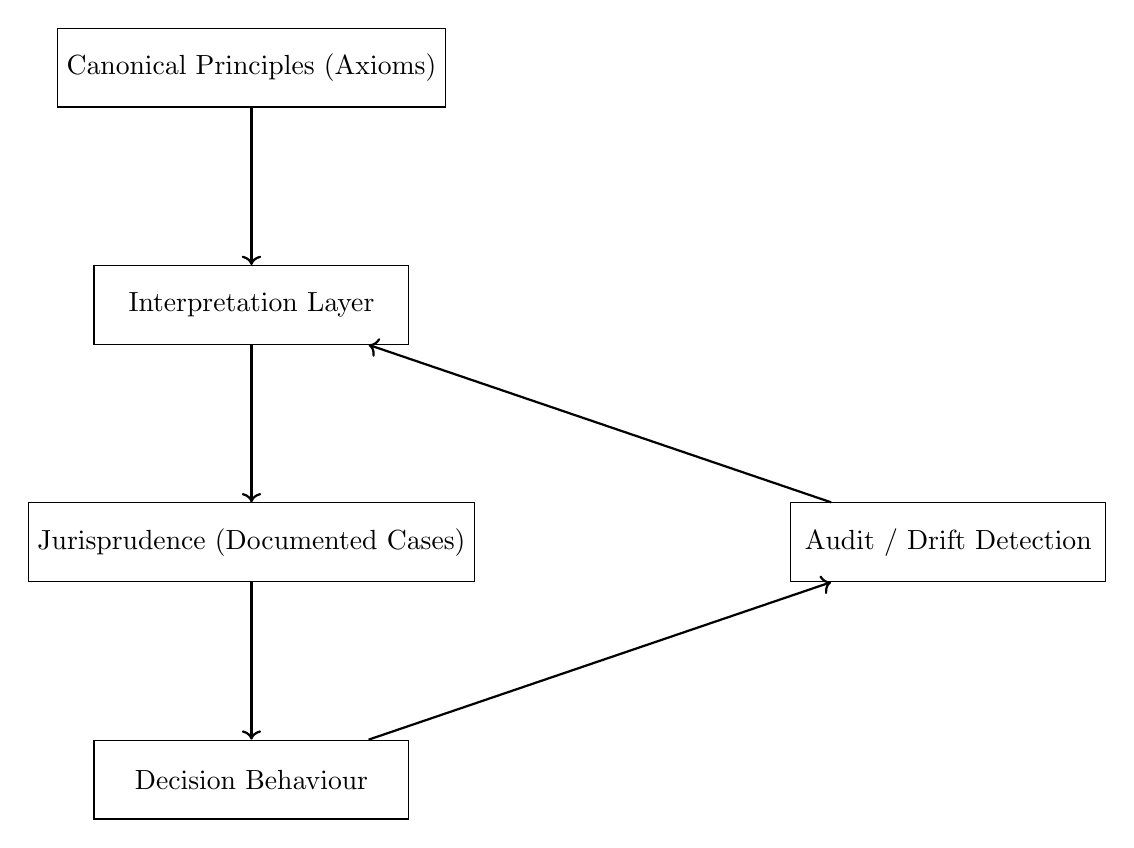
\begin{tikzpicture}[
node distance=2cm,
box/.style={rectangle, draw, minimum width=4cm, minimum height=1cm},
arrow/.style={->, thick}
]

\node[box] (canon) {Canonical Principles (Axioms)};
\node[box, below=of canon] (interpretation) {Interpretation Layer};
\node[box, below=of interpretation] (jurisprudence) {Jurisprudence (Documented Cases)};
\node[box, below=of jurisprudence] (decision) {Decision Behaviour};

\node[box, right=4cm of jurisprudence] (audit) {Audit / Drift Detection};

\draw[arrow] (canon) -- (interpretation);
\draw[arrow] (interpretation) -- (jurisprudence);
\draw[arrow] (jurisprudence) -- (decision);

\draw[arrow] (decision) -- (audit);
\draw[arrow] (audit) -- (interpretation);

\end{tikzpicture}

\end{center}

\section{Conclusion}

Optimisation-based alignment systems are adaptive by design. Adaptation without fixed structural boundaries produces drift.

A constitutional constraint architecture introduces a stable normative anchor. It separates immutable principles from contextual interpretation and makes drift detectable rather than invisible.

The proposal does not claim perfection. It proposes structural stabilisation as an alternative foundation for alignment design.

Rather than treating ethical principles as variables within an optimisation process, the framework treats certain principles as boundaries that define the permissible space of action.

In this sense, the model attempts to replace value optimisation with boundary-based alignment.

\bibliographystyle{plain}

\begin{thebibliography}{9}

\bibitem{christiano2017preferences}
Paul Christiano, Jan Leike, Tom Brown, et al.
\newblock Deep Reinforcement Learning from Human Preferences.
\newblock In \textit{Advances in Neural Information Processing Systems}, 2017.

\bibitem{bai2022constitutional}
Yuntao Bai, Andy Jones, Kamal Ndousse, et al.
\newblock Constitutional AI: Harmlessness from AI Feedback.
\newblock Anthropic, 2022.

\bibitem{amodei2016concrete}
Dario Amodei, Chris Olah, Jacob Steinhardt, et al.
\newblock Concrete Problems in AI Safety.
\newblock arXiv:1606.06565, 2016.

\bibitem{russell2019humancompatible}
Stuart Russell.
\newblock \textit{Human Compatible: Artificial Intelligence and the Problem of Control}.
\newblock Viking Press, 2019.

\end{thebibliography}

\end{document}
